% =====================================================================
% EXPANDED RESULTS SECTION (replaces the short \section{Controlled Result})
% =====================================================================
\section{Results}
\label{sec:main}

\begin{figure}[t]
\centering
\begin{tikzpicture}
\begin{axis}[width=0.92\linewidth,height=5.2cm,xlabel={layer},ylabel={between-dialogue spread},ymin=0, xmin=1,xmax=24,grid=both,grid style={line width=.2pt,draw=gray!18},major grid style={line width=.3pt,draw=gray!30},tick align=outside,tick style={gray!50},axis line style={gray!55},legend style={font=\footnotesize,draw=gray!40,fill=white,fill opacity=0.85,text opacity=1},legend cell align=left,legend pos=north east,label style={font=\small},tick label style={font=\footnotesize}]
\addplot[draw=none,name path=lor] coordinates {(1,0.419) (2,0.374) (3,0.356) (4,0.304) (5,0.297) (6,0.402) (7,0.312) (8,0.268) (9,0.260) (10,0.233) (11,0.245) (12,0.267) (13,0.231) (14,0.244) (15,0.239) (16,0.197) (17,0.202) (18,0.201) (19,0.215) (20,0.199) (21,0.202) (22,0.211) (23,0.218) (24,0.222)};
\addplot[draw=none,name path=hir] coordinates {(1,0.669) (2,0.500) (3,0.476) (4,0.424) (5,0.409) (6,0.499) (7,0.378) (8,0.338) (9,0.334) (10,0.297) (11,0.371) (12,0.471) (13,0.401) (14,0.415) (15,0.406) (16,0.321) (17,0.321) (18,0.319) (19,0.326) (20,0.313) (21,0.305) (22,0.312) (23,0.323) (24,0.326)};
\addplot[blue!55,opacity=0.18,forget plot] fill between[of=lor and hir];
\addplot[draw=none,name path=los] coordinates {(1,0.565) (2,0.384) (3,0.369) (4,0.320) (5,0.340) (6,0.428) (7,0.332) (8,0.308) (9,0.299) (10,0.241) (11,0.255) (12,0.287) (13,0.236) (14,0.244) (15,0.235) (16,0.187) (17,0.184) (18,0.185) (19,0.195) (20,0.188) (21,0.195) (22,0.195) (23,0.204) (24,0.202)};
\addplot[draw=none,name path=his] coordinates {(1,0.734) (2,0.534) (3,0.513) (4,0.459) (5,0.443) (6,0.529) (7,0.398) (8,0.356) (9,0.343) (10,0.296) (11,0.340) (12,0.371) (13,0.338) (14,0.349) (15,0.317) (16,0.272) (17,0.279) (18,0.275) (19,0.292) (20,0.296) (21,0.295) (22,0.314) (23,0.312) (24,0.313)};
\addplot[orange!70,opacity=0.18,forget plot] fill between[of=los and his];
\addplot[blue!70!black,thick,mark=*,mark size=1.1pt] coordinates {(1,0.598) (2,0.428) (3,0.414) (4,0.360) (5,0.359) (6,0.451) (7,0.352) (8,0.309) (9,0.308) (10,0.264) (11,0.323) (12,0.347) (13,0.317) (14,0.327) (15,0.323) (16,0.245) (17,0.250) (18,0.253) (19,0.268) (20,0.266) (21,0.261) (22,0.264) (23,0.270) (24,0.275)};
\addlegendentry{real dialogues}
\addplot[orange!75!black,thick,densely dashed,mark=square*,mark size=1.1pt] coordinates {(1,0.658) (2,0.445) (3,0.422) (4,0.366) (5,0.359) (6,0.471) (7,0.371) (8,0.332) (9,0.323) (10,0.267) (11,0.291) (12,0.322) (13,0.287) (14,0.302) (15,0.272) (16,0.219) (17,0.222) (18,0.221) (19,0.235) (20,0.231) (21,0.241) (22,0.249) (23,0.251) (24,0.240)};
\addlegendentry{scrambled twins}
\end{axis}
\end{tikzpicture}
\caption{Controlled result ($n{=}12$ dialogues, dialogue-level 95\% CIs). Real (blue) and
scrambled-twin (orange) between-dialogue spread bands overlap at every layer: coherent
content adds nothing detectable beyond the length/topic that the scrambled twin already
matches. Compare to the $n{=}3$ placebo (Figure~\ref{fig:placebo}), which appeared
positive.}
\label{fig:scaled}
\end{figure}

\begin{figure}[t]
\centering
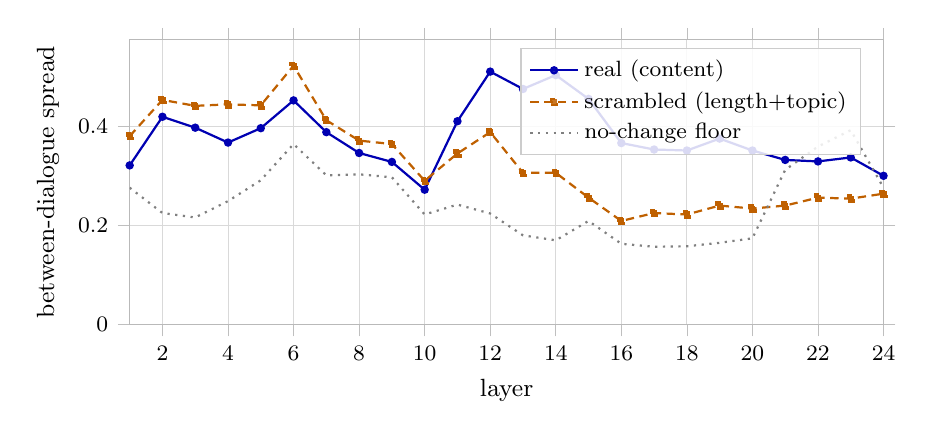
\begin{tikzpicture}
\begin{axis}[width=0.92\linewidth,height=5.2cm,xlabel={layer},ylabel={between-dialogue spread},ymin=0, xmin=1,xmax=24,grid=both,grid style={line width=.2pt,draw=gray!18},major grid style={line width=.3pt,draw=gray!30},tick align=outside,tick style={gray!50},axis line style={gray!55},legend style={font=\footnotesize,draw=gray!40,fill=white,fill opacity=0.85,text opacity=1},legend cell align=left,legend pos=north east,label style={font=\small},tick label style={font=\footnotesize}]
\addplot[blue!70!black,thick,mark=*,mark size=1.1pt] coordinates {(1,0.321) (2,0.419) (3,0.397) (4,0.367) (5,0.396) (6,0.452) (7,0.388) (8,0.346) (9,0.328) (10,0.272) (11,0.410) (12,0.510) (13,0.475) (14,0.503) (15,0.455) (16,0.366) (17,0.353) (18,0.351) (19,0.375) (20,0.351) (21,0.332) (22,0.329) (23,0.337) (24,0.300)};
\addlegendentry{real (content)}
\addplot[orange!75!black,thick,densely dashed,mark=square*,mark size=1.1pt] coordinates {(1,0.380) (2,0.453) (3,0.441) (4,0.444) (5,0.442) (6,0.522) (7,0.412) (8,0.371) (9,0.364) (10,0.290) (11,0.345) (12,0.388) (13,0.306) (14,0.306) (15,0.256) (16,0.209) (17,0.225) (18,0.222) (19,0.240) (20,0.234) (21,0.240) (22,0.256) (23,0.254) (24,0.264)};
\addlegendentry{scrambled (length+topic)}
\addplot[gray,dotted,thick] coordinates {(1,0.276) (2,0.225) (3,0.216) (4,0.249) (5,0.291) (6,0.364) (7,0.301) (8,0.303) (9,0.297) (10,0.222) (11,0.242) (12,0.224) (13,0.180) (14,0.170) (15,0.209) (16,0.163) (17,0.157) (18,0.158) (19,0.165) (20,0.174) (21,0.312) (22,0.359) (23,0.392) (24,0.276)};
\addlegendentry{no-change floor}
\end{axis}
\end{tikzpicture}
\caption{The $n{=}3$ placebo that the controlled result overturns. Early layers (1--10):
scrambled $\geq$ real (a length/lexical artifact). Mid-late layers (11--21): real $>$
scrambled, which \emph{looked} like a content effect but, lacking a dialogue-level CI,
was a small-sample artifact (Figure~\ref{fig:scaled}).}
\label{fig:placebo}
\end{figure}

\begin{figure}[t]
\centering
\begin{tikzpicture}
\begin{axis}[width=0.92\linewidth,height=5.2cm,xlabel={layer},ylabel={re-entanglement leak $d(H_1,H_t)$},ymin=0, xmin=1,xmax=24,grid=both,grid style={line width=.2pt,draw=gray!18},major grid style={line width=.3pt,draw=gray!30},tick align=outside,tick style={gray!50},axis line style={gray!55},legend style={font=\footnotesize,draw=gray!40,fill=white,fill opacity=0.85,text opacity=1},legend cell align=left,legend pos=north east,label style={font=\small},tick label style={font=\footnotesize}]
\addplot[draw=none,name path=lor] coordinates {(1,0.285) (2,0.368) (3,0.402) (4,0.484) (5,0.571) (6,0.594) (7,0.478) (8,0.409) (9,0.422) (10,0.328) (11,0.366) (12,0.418) (13,0.326) (14,0.361) (15,0.317) (16,0.272) (17,0.276) (18,0.282) (19,0.306) (20,0.291) (21,0.286) (22,0.289) (23,0.295) (24,0.284)};
\addplot[draw=none,name path=hir] coordinates {(1,0.538) (2,0.482) (3,0.485) (4,0.550) (5,0.594) (6,0.621) (7,0.516) (8,0.431) (9,0.437) (10,0.355) (11,0.402) (12,0.459) (13,0.372) (14,0.414) (15,0.375) (16,0.340) (17,0.365) (18,0.378) (19,0.416) (20,0.400) (21,0.380) (22,0.411) (23,0.423) (24,0.426)};
\addplot[blue!55,opacity=0.18,forget plot] fill between[of=lor and hir];
\addplot[draw=none,name path=los] coordinates {(1,0.326) (2,0.321) (3,0.373) (4,0.486) (5,0.561) (6,0.602) (7,0.508) (8,0.438) (9,0.462) (10,0.361) (11,0.372) (12,0.420) (13,0.319) (14,0.322) (15,0.271) (16,0.234) (17,0.236) (18,0.235) (19,0.250) (20,0.241) (21,0.225) (22,0.230) (23,0.235) (24,0.229)};
\addplot[draw=none,name path=his] coordinates {(1,0.461) (2,0.472) (3,0.495) (4,0.566) (5,0.630) (6,0.651) (7,0.561) (8,0.479) (9,0.487) (10,0.385) (11,0.443) (12,0.490) (13,0.367) (14,0.378) (15,0.324) (16,0.283) (17,0.277) (18,0.282) (19,0.298) (20,0.295) (21,0.284) (22,0.295) (23,0.299) (24,0.288)};
\addplot[orange!70,opacity=0.18,forget plot] fill between[of=los and his];
\addplot[blue!70!black,thick,mark=*,mark size=1.1pt] coordinates {(1,0.354) (2,0.445) (3,0.457) (4,0.532) (5,0.582) (6,0.608) (7,0.500) (8,0.423) (9,0.432) (10,0.344) (11,0.390) (12,0.437) (13,0.349) (14,0.383) (15,0.356) (16,0.307) (17,0.336) (18,0.344) (19,0.367) (20,0.357) (21,0.347) (22,0.363) (23,0.377) (24,0.380)};
\addlegendentry{real dialogues}
\addplot[orange!75!black,thick,densely dashed,mark=square*,mark size=1.1pt] coordinates {(1,0.383) (2,0.420) (3,0.436) (4,0.536) (5,0.610) (6,0.629) (7,0.525) (8,0.464) (9,0.475) (10,0.373) (11,0.392) (12,0.449) (13,0.353) (14,0.362) (15,0.313) (16,0.258) (17,0.254) (18,0.257) (19,0.271) (20,0.266) (21,0.258) (22,0.263) (23,0.261) (24,0.259)};
\addlegendentry{scrambled twins}
\end{axis}
\end{tikzpicture}
\caption{The static disentangling projector (fit at turn 1) re-entangles substantially by
turn 4 (leak $d(H_1,H_4)$, blue), but its length/topic-matched scrambled twin (orange) leaks
just as much: the static baseline's apparent failure is a length/topic artifact, not
content-driven, so a content-conditional projector would not fix it.}
\label{fig:static}
\end{figure}

We report results in five movements. We first validate the estimator and decision rule
against analytic ground truth (\S\ref{sec:res-synth}), then fix the operating point with a
power analysis (\S\ref{sec:res-power}). We then walk the rigor cascade, three intuitive
positive measurements each overturned by the next control (\S\ref{sec:res-cascade}), before
presenting the controlled result and its cross-model and SAE-feature-space replications
(\S\ref{sec:res-controlled}). Finally we fit the static disentangling projector these methods
would replace and show its apparent failure is itself a confound (\S\ref{sec:res-static}).
Every number below is from a run on the released code; the synthetic checks of
\S\ref{sec:res-synth} require no model and reproduce anywhere. Throughout, the
pre-registered decision rule is: a layer is content-conditional iff the real
between-dialogue spread's $95\%$ CI lower bound exceeds the scrambled-twin spread's $95\%$ CI
upper bound, and the verdict is \textsc{content\_conditional} iff a contiguous band of
$\geq 3$ such layers exists.

\subsection{Synthetic validation: the estimator recovers known geometry}
\label{sec:res-synth}

Before touching a model we confirm that the pipeline measures what it claims to. We build
paired activations whose contrast subspace is an analytically controlled object and check
that the estimator and the decision rule behave correctly in three regimes
(Table~\ref{tab:synth}). With a known $15^\circ$/turn rotation injected into the contrast
subspace, the noise-corrected chordal drift is $0.144$ against the analytic value $0.149$, and the decision rule fires positive. With a static (zero-rotation)
subspace the measured drift collapses to the bootstrap noise floor and the rule correctly
returns negative, the property that protects against calling an under-powered run a real
effect. The principal-angle routine returns $0$ for identical planes and $\pi/2$ for
orthogonal ones, confirming the gauge-invariant geometry is implemented correctly. The same
code path is used for every real run below, so a real verdict reflects the data and not a
code artifact.

\begin{table}[t]
\centering
\small
\begin{tabular}{@{}llll@{}}
\toprule
Ground-truth construction & Quantity & Measured & Expected / verdict \\
\midrule
$15^\circ$/turn injected rotation & noise-corrected drift & $0.144$ & $0.149$ (analytic) \\
static (zero-rotation) subspace & drift & at bootstrap floor & negative (correct) \\
identical planes & principal angle & $0$ & $0$ \\
orthogonal planes & principal angle & $\pi/2$ & $\pi/2$ \\
\bottomrule
\end{tabular}
\caption{Synthetic validation against analytic ground truth (no model, no network). The
estimator recovers an injected rotation accurately ($0.144$ vs.\ $0.149$), returns the bootstrap floor (a
correct negative) for a static subspace, and passes the principal-angle sanity checks.}
\label{tab:synth}
\end{table}

\subsection{Power analysis: rank-1 and $\geq 96$ probes}
\label{sec:res-power}

Subspace estimation in $d\!\approx\!10^3$ activation space is noisy, and the bootstrap noise
floor (the drift between two resamples of the \emph{same} subspace) sets the smallest effect
the protocol can resolve. On \texttt{Qwen2.5-0.5B-Instruct} (raw activations, rank-1) the
$95\%$ floor falls from $0.49$ at $16$ probes to $0.22$ at $96$ probes, scaling as
$\approx 1/\sqrt{n_{\text{probes}}}$ (Table~\ref{tab:power}). Higher-rank subspaces are not
usable at these sample sizes: a rank-2 or rank-3 fit from a few dozen probes returns a floor
of $\approx 0.7$, meaning two estimates of the \emph{same} subspace are nearly orthogonal, so
the recovered directions are noise. We therefore operate at rank-1 with $\geq 96$ probe pairs
per side, and we report the floor alongside every drift so that a null is never mistaken for
an under-powered run.

Power is summarized in Table~\ref{tab:power} (Section~\ref{sec:power}).

\subsection{The rigor cascade: three positive measurements, each overturned}
\label{sec:res-cascade}\label{sec:cascade}

We arrived at the controlled result through a sequence of measurements of increasing rigor,
each of which caught a confound in the previous one (Table~\ref{tab:cascade}). We present the
cascade in full because it is itself a contribution: it shows concretely how intuitive
measurements of representational drift produce false positives, and which control removes each.

\begin{table}[t]
\centering
\small
\begin{tabular}{@{}llll@{}}
\toprule
Step & Measurement & Headline & Overturned by \\
\midrule
1 & consecutive drift, 32 probes, one layer & inconclusive (under-powered) & noise floor too high \\
2 & cumulative drift from turn 0 & \textcolor{red}{positive} & turn-0 onset confound \\
3 & spread vs same-context floor & \textcolor{red}{positive} (21 layers) & floor carries no length variance \\
4 & scrambled placebo, $n{=}3$ dialogues & \textcolor{red}{positive} (layers 11--21) & $n{=}3$, no CI; one outlier dialogue \\
5 & \textbf{scrambled, $n{=}12$, dialogue-level CI} & \textbf{negative} & (the controlled result) \\
\bottomrule
\end{tabular}
\caption{Each row's headline was overturned by the next control. Steps 2--4 are \emph{false
positives} produced by intuitive but confounded measurements; step 5 is the controlled result
reported in \S\ref{sec:res-controlled}.}
\label{tab:cascade}
\end{table}

\paragraph{Step 1 (under-power).} A consecutive-turn drift with only $32$ probes at a single
layer is inconclusive: the noise floor at $32$ probes ($0.31$, Table~\ref{tab:power}) is
comparable to any motion present, so nothing can be concluded. This is why power must be fixed
first.

\paragraph{Step 2 (no-context onset, a false positive).} Measuring cumulative drift from turn
$0$ produces a large, apparently positive signal. The tell is that the between-dialogue spread
($\approx 0.37$) is far below the turn-$0$ displacement ($\approx 0.88$): almost all of the
motion is the generic bare-probe$\to$probe-in-context jump, which is shared across dialogues
and is not content-conditional. Baselining at turn $1$ and measuring $d(U_1,U_t)$ removes it.

\paragraph{Step 3 (same-context floor, a false positive over 21 layers).} Comparing the
between-dialogue spread against a same-context resampling floor looks positive at $21$ layers,
but this comparison is near-tautological. The floor resamples probes within one fixed context
and therefore contains zero between-dialogue length, topic, and position variance, while the
spread contains all of it. Empirically the between-dialogue spread grew monotonically with
turn index in lockstep with the per-turn token-length gap, which widened from $3$ to $20$
tokens across turns ($\approx 12\%$ at the turn where the spread is measured): the signature
of a length artifact, not of content.

\paragraph{Step 4 (small-sample placebo, a false positive at layers 11--21).} Introducing the
scrambled-twin null with $n{=}3$ dialogues appears to rescue a content effect at the
mid-to-late layers (layers $11$--$21$, real $>$ scrambled; Figure~\ref{fig:placebo}). But this
is a point estimate with no confidence interval, and its median rests on a single
topically-divergent dialogue. Resampling at the dialogue level dissolves it.

\paragraph{Step 5 (the controlled result).} With $n{=}12$ dialogues, the scrambled-twin null,
and a dialogue-level bootstrap CI, the verdict is negative. This is the controlled measurement
we report next.

\subsection{Controlled result and replications}
\label{sec:res-controlled}

\paragraph{Model and data.} We report \texttt{Qwen2.5-0.5B-Instruct} \citep{qwen25}
($896$-dim residual stream, $24$ layers), rank-1 difference-of-means directions, $64$--$96$
probe pairs per side, and $12$ topically diverse $5$-turn dialogues. For the headline test we
take each dialogue's final-turn (full-context) hallucination subspace $H_t$ at every layer,
compute the median pairwise between-dialogue chordal spread, and bracket it with a
dialogue-level bootstrap $95\%$ CI, against the length- and topic-matched scrambled-twin null.

\paragraph{The hallucination subspace is not content-conditional on this model.} The apparent
content-conditionality does not survive (Figure~\ref{fig:scaled}, Table~\ref{tab:qwen05}). At
\emph{every} layer the real-dialogue spread CI overlaps the scrambled-twin spread CI: at layer
$12$, real $0.347$ $[0.27,0.47]$ versus scrambled $0.322$ $[0.29,0.37]$; at layer $15$, real
$0.323$ $[0.24,0.41]$ versus scrambled $0.272$ $[0.24,0.32]$. A small, consistent,
non-significant trend remains at the mid-to-late layers (real slightly above scrambled), but no
layer satisfies the decision rule (real CI lower bound $>$ scrambled CI upper bound), so no
contiguous band exists and the verdict is \textsc{not\_content\_conditional}. Scrambled twins,
which hold token length, position, and lexical topic fixed while destroying coherent dialogue
meaning, move the hallucination subspace as much as the real dialogues do. The between-dialogue
movement is therefore attributable to length and topic, not to coherent dialogue content.

\begin{table}[t]
\centering
\small
\begin{tabular}{@{}lccc@{}}
\toprule
Layer & Real spread $[95\%\ \text{CI}]$ & Scrambled spread $[95\%\ \text{CI}]$ & Clears rule? \\
\midrule
$12$ & $0.347$ $[0.27,0.47]$ & $0.322$ $[0.29,0.37]$ & no \\
$15$ & $0.323$ $[0.24,0.41]$ & $0.272$ $[0.24,0.32]$ & no \\
\bottomrule
\end{tabular}
\caption{Controlled result on \texttt{Qwen2.5-0.5B-Instruct} (raw activations, $24$ layers,
$n{=}12$ dialogues, rank-1, dialogue-level bootstrap). Representative mid-late layers: real and
scrambled-twin CIs overlap, no layer clears the decision rule, and no $\geq 3$-contiguous band
forms. Verdict: \textsc{not\_content\_conditional}.}
\label{tab:qwen05}
\end{table}

\paragraph{The safety side is worse, not better.} The premise that matters for conditional
\emph{disentanglement} concerns the joint geometry of $S_t$ and $H_t$. On this model the
refusal direction is not cleanly recoverable below the mid layers: two independent estimates of
the same $S$ subspace are near-orthogonal (floor $\approx 1.0$) through roughly the first half
of the network, becoming recoverable only at the later layers. The cross-subspace overlap
$\Omega(S_t,H_t)$ is therefore meaningful only at late layers, where its movement across turns
is small. We thus cannot even measure the entanglement drift that conditional disentanglement
is designed to track, let alone show it is large.

\paragraph{Replication across model scale (Qwen2.5-1.5B).} The same controlled test on
\texttt{Qwen2.5-1.5B-Instruct} ($28$ layers, $n{=}12$, rank-1) returns the same verdict: the
content-conditional band is empty (Table~\ref{tab:qwen15}). At layer $1$, real $0.653$
$[0.56,0.69]$ versus scrambled $0.665$ $[0.57,0.72]$; at the late layers real slightly exceeds
scrambled but the CIs overlap throughout, so no layer clears the rule. The null is therefore
not an artifact of the smallest model.

\begin{table}[t]
\centering
\small
\begin{tabular}{@{}lccc@{}}
\toprule
Layer & Real spread $[95\%\ \text{CI}]$ & Scrambled spread $[95\%\ \text{CI}]$ & Clears rule? \\
\midrule
$1$ & $0.653$ $[0.56,0.69]$ & $0.665$ $[0.57,0.72]$ & no \\
late layers & real slightly $>$ scrambled & CIs overlap throughout & no \\
\bottomrule
\end{tabular}
\caption{Cross-scale replication on \texttt{Qwen2.5-1.5B-Instruct} (raw activations, $28$
layers, $n{=}12$, rank-1). The content-conditional band is empty; verdict
\textsc{not\_content\_conditional}.}
\label{tab:qwen15}
\end{table}

\paragraph{Replication in SAE feature space (GPT-2 small).} Because disentanglement methods
operate on SAE features rather than raw activations, we repeated the controlled test in the
feature space of GPT-2 small using the publicly released residual-stream SAEs at all twelve
layers \citep{cunningham2023sparse, bricken2023monosemanticity}, encoding each contrastive
probe's last-token activation through the frozen SAE and recovering $H_t$ in feature
coordinates. The verdict is unchanged: at no layer does the real between-dialogue spread clear
the scrambled-twin spread, the band is empty, and at the late layers ($7$--$11$), where
abstract features concentrate, the scrambled spread is in fact \emph{larger} than the real
spread (Table~\ref{tab:gpt2sae}). At layer $10$, real $0.515$ $[0.46,0.58]$ versus scrambled
$0.659$ $[0.58,0.80]$; at layer $11$, real $0.541$ $[0.47,0.64]$ versus scrambled $0.668$
$[0.59,0.74]$. The apparent context-dependence is, if anything, \emph{better} explained by
length and lexical content in feature space than in raw space. The null is thus not an artifact
of the activation basis: it holds in the exact representation conditional disentanglement would
use.

\begin{table}[t]
\centering
\small
\begin{tabular}{@{}lccc@{}}
\toprule
Layer & Real spread $[95\%\ \text{CI}]$ & Scrambled spread $[95\%\ \text{CI}]$ & Scrambled $>$ real? \\
\midrule
$10$ & $0.515$ $[0.46,0.58]$ & $0.659$ $[0.58,0.80]$ & yes \\
$11$ & $0.541$ $[0.47,0.64]$ & $0.668$ $[0.59,0.74]$ & yes \\
\bottomrule
\end{tabular}
\caption{SAE-feature-space replication on GPT-2 small (\texttt{gpt2-small-res-jb} residual
SAEs, all $12$ layers, $n{=}12$, rank-1). The band is empty, and at the late layers the
scrambled-twin spread \emph{exceeds} the real spread: length and lexical content explain the
movement at least as well as coherent content. Verdict \textsc{not\_content\_conditional}.}
\label{tab:gpt2sae}
\end{table}

\subsection{Demonstration: the static baseline does not genuinely fail}
\label{sec:res-static}

The premise's operational consequence is that a \emph{static} disentangling projector, fit
once, should fail at later turns, which is what motivates replacing it with a conditional one.
We test this directly on \texttt{Qwen2.5-0.5B-Instruct} ($n{=}12$). The static projector built
at turn $1$ nulls the hallucination subspace $H_1$; its residual re-entanglement leak at turn
$t$, the fraction of $H_t$ the frozen projector fails to remove, is exactly $d(H_1,H_t)\in[0,1]$,
while a conditional projector rebuilt at turn $t$ has leak $0$ by construction. Naively the
static projector looks broken: its leak by turn $4$ is large, $0.3$--$0.6$ across layers
(Figure~\ref{fig:static}). But the length- and topic-matched scrambled twins leak \emph{just as
much} (Table~\ref{tab:static}): at layer $8$, real $0.423$ $[0.41,0.43]$ versus scrambled
$0.464$ $[0.44,0.48]$; at layer $12$, real $0.437$ versus scrambled $0.449$. Only $3$ of $25$
layers (all late: $18$, $19$, $21$) show real leak exceeding scrambled at the dialogue-level
$95\%$ level, and they are not contiguous, below our pre-registered $\geq 3$-contiguous-layer
rule and near the $\approx 1.25$ layers expected by chance. We report this weak, non-robust
late-layer elevation rather than hide it. The verdict is \textsc{static\_failure\_is\_confound}:
for this behavior and model, a static projector's degradation across turns is confound-explained,
so a content-conditional projector would not fix it and the conditional machinery addresses a
confound rather than a real non-stationarity.

\begin{table}[t]
\centering
\small
\begin{tabular}{@{}lccc@{}}
\toprule
Layer & Real leak $d(H_1,H_t)$ $[95\%\ \text{CI}]$ & Scrambled leak $[95\%\ \text{CI}]$ & Real $>$ scrambled? \\
\midrule
$8$ & $0.423$ $[0.41,0.43]$ & $0.464$ $[0.44,0.48]$ & no \\
$12$ & $0.437$ & $0.449$ & no \\
\midrule
\multicolumn{4}{@{}l}{Only $3/25$ layers (late: $18,19,21$) cross the dialogue-level bar; \emph{not} contiguous ($\geq 3$ rule unmet; chance $\approx 1.25$).} \\
\bottomrule
\end{tabular}
\caption{Static-projector demonstration on \texttt{Qwen2.5-0.5B-Instruct} ($n{=}12$). The
static projector's apparent across-turn re-entanglement is matched by its length/topic
scrambled twin, so it does not genuinely fail. Verdict \textsc{static\_failure\_is\_confound}.}
\label{tab:static}
\end{table}

\paragraph{Summary across settings.} Every configuration tested under the full protocol
(\texttt{Qwen2.5-0.5B-Instruct} and \texttt{Qwen2.5-1.5B-Instruct} in raw activation space, and
GPT-2 small in SAE feature space) returns \textsc{not\_content\_conditional}, and the
static-projector demonstration returns \textsc{static\_failure\_is\_confound}. On the
instruction-tuned and GPT-2 models we evaluate, in raw and SAE feature space, the apparent
context-conditionality of the hallucination subspace is statistically indistinguishable from a
length and topic artifact.

% =====================================================================
% REPRODUCIBILITY APPENDIX
% =====================================================================
